\chapter{Theoretical Background}
\label{cha:theoreticalBackground}
    %
    %

    %
    \section{Chemical master equation}
        \label{subsec:CME}
        %
        %
        The chemical master equation (CME) (see \ref{eqn:CME}, taken from \cite{johnson2021quantifying}) takes the discrete and stochastic nature of a (bio)chemical system into account. It describes the time-dependent evolution of a homogenous system's change in state based on reaction probabilities \cite{Ge2013, johnson2021quantifying}.

        \begin{equation}
            \frac{dP(N,t)}{dt} = \sum^{R}_{r}{\alpha_r (N -\nu_r) \times P(N-\nu_r, t)} - \sum^{R}_{r}{\alpha_r(N) \times P(N,t)}
            \label{eqn:CME}
        \end{equation}

        %
        The CME consists of coupled ordinary differential equations and describes the time $t$ dependent probability $P$ to occupy one state $P(N,t)$ of a discrete set of states. $N$ is a composition vector describing the abundance of each chemical species. $R$ denotes the number of all possible reactions $r$. $\nu_r$ is the stoichiometric vector that thus describes the change of the number of every chemical species in $N$ if the system undergoes reaction $r$. $\alpha_r$ indicates the probability per unit time that $r$ can occur.
        %

        %
        Analytical solutions of the CME are rarely used in practical models, especially in biological systems \cite{johnson2021quantifying} because of the high computational complexity in real-life inspired models, as solving the CME scales exponentially with the number of different chemical entities in the system.
    %
    %
    \section{Dynamic histone PTM models}
        %

        %
        In order to establish the CME for a histone PTM model, one can establish the modification concentration dependent differential equation \cite{lemons1908paper} for each modification type with respect to the HME types that take part in changing the respective modification concentration.
        %

        %
        For practical illustration, consider a histone PTM model which includes two mutually-exclusive modifications: acetylation (\ac/) and methylation (\me/) of nucleosomes. The nucleosomes are not distinguishable from one another apart from being either acetylated, methylated or unmodified. The HMEs contained in the system are \ac/ writers, \ac/ removers, \me/ writers and \me/ removers.
        %

        %
        The CME for such a system was already formed and analysed by Mayer in \cite{mayer2020langevin}.
        %

        %
        Eqns. \ref{eqn:noncooperative} describe the CME for $a = \frac{A}{N}$ and $m = \frac{M}{N}$ with $A$ the number of acetylated nucleosomes, $M$ the number of methylated nucleosomes and $N$ the total number of nucleosomes. $\alpha_i$ and $\beta_i$ are probability coefficients taking into account the types, association and dissociation rates of the enzymes in the system.
        %

        %
        \begin{subequations}
            \begin{align}
                &\frac{\partial a}{\partial t} = \underbrace{- \alpha_1 a }_{\textrm{ac removal}} + \underbrace{ \alpha_2 a (1-a-m) }_{\textrm{ac addition}}\\
                &\frac{\partial m}{\partial t} = \underbrace{- \beta_1 m }_{\textrm{me removal}} + \underbrace{ \beta_2 m (1-a-m) }_{\textrm{me addition}}
            \end{align}
            \label{eqn:noncooperative}
        \end{subequations}
        %

        %
        It is important to note that $a$ and $m$ describe the relative number of the corresponding modification among the nucleosomes which implies that every nucleosome with a specific type of modification is one chemical species. If one considers a system in which nucleosomes have one and the same neighbour the entire time one could define enzymatic reactions that take these fixed neighbour relations into account.
        %

        %
        An appropriate CME model would then require to establish and solve the CME for every nucleosome while the CME for nucleosome $i$ would depend on the number of next-neighbours equal to the biggest enzyme reading frame in the system. For instance, if the enzyme only considers the next neighbours $i+1$ and $i-1$ of the nucleosome $i$ to be modified, the CME system would change to eqns. \ref{eqn:neighbourDependent}.
        %

        %
        \begin{subequations}
            \begin{align}
                &\frac{\partial a_i}{\partial t} = - \alpha_1 (a_{i-1} + a_i + a_{i+1}) + \alpha_2 (a_{i-1} + a_i + a_{i+1}) \times (1-a-m)\\
                &\frac{\partial m_i}{\partial t} = - \beta_1 (m_{i-1} + m_i + m_{i+1}) + \beta_2 (m_{i-1} + m_i + m_{i+1}) \times (1-a-m)
            \end{align}
            \label{eqn:neighbourDependent}
        \end{subequations}
        %

        %
        This differential equation system quickly increases in complexity and dimensionality with increasing number of nucleosomes in the system and higher reach of the enzymes up to a point where an analytical solution is impossible to achieve. Mainly for this reason, it is convenient to numerically simulate the time-dependent evolution of the system.
        %
        %
    %
    \section{Stochastic simulation algorithm}
    \label{subsec:Gillespie}
        %
        Gillespie's \textit{stochastic simulation algorithm} (SSA) simulates the evolution in time of a spatially homogenous molecular mixture with a discrete number of reactants under specification of the coupled reaction channels based on stochastic chemical kinetics \cite{gillespie1976general, gillespie1992rigorous}. This is useful especially when the practice of solving the chemical master equation analytically is not ideal.
        %

        %
        Gillespie takes an event-based time step approach. This ensures that at every time step, exactly one event is taking place. This approach obviously reduces the overhead compared to an equidistant time step approach (see fig. \ref{img:Gillespie_timeSteps}) and can massively facilitate implementation and later interpretation of the simulation results.
        %

        %
        \begin{figure}[htpb!]
            \centering
            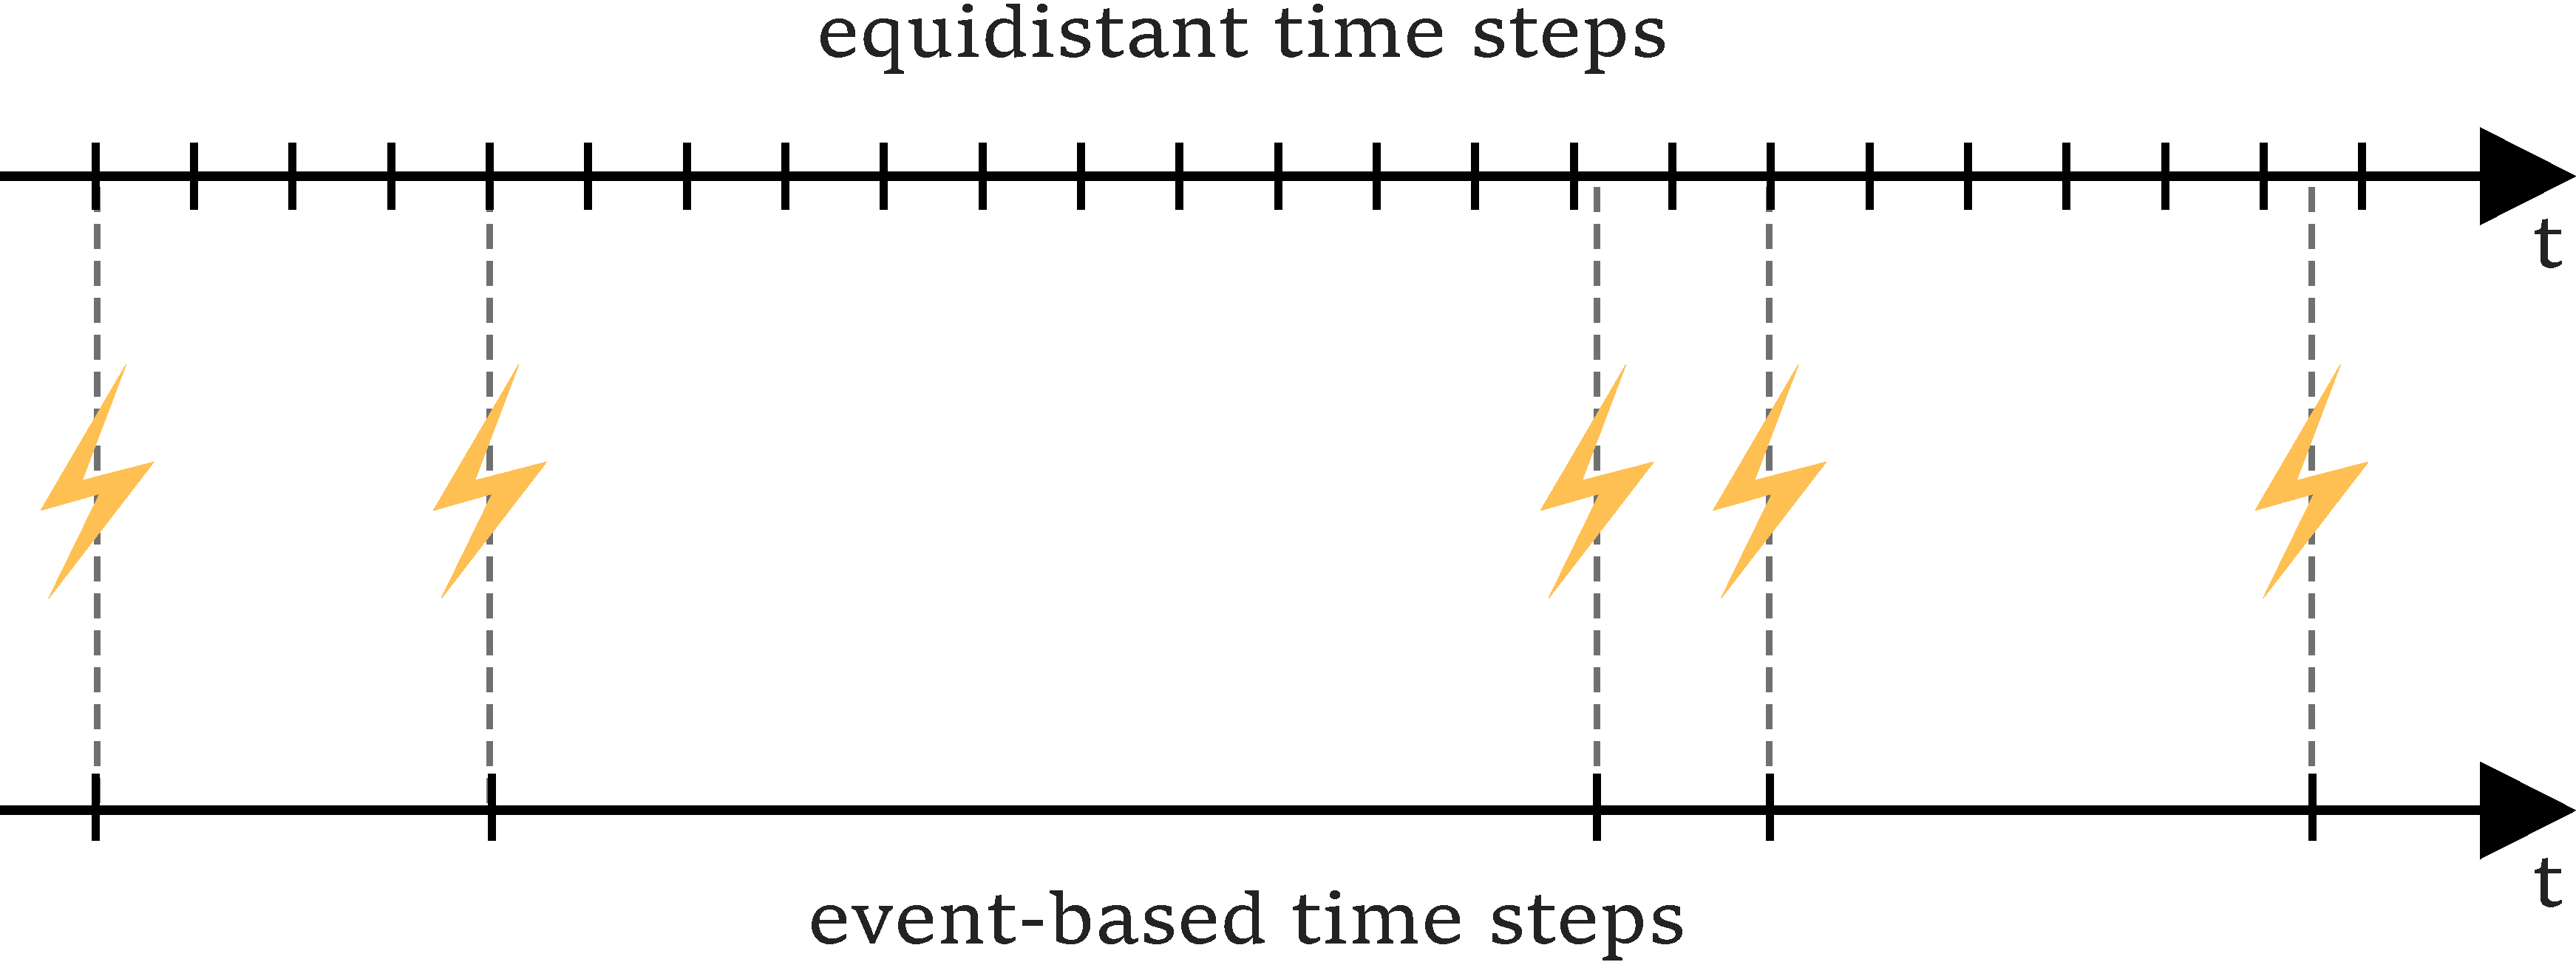
\includegraphics[width=0.7\textwidth]{Gillespie_timeSteps.pdf}
            \caption{Schematic illustration of equidistant time steps vs. event-based time steps inspired by Mayer in \cite{mayer2020langevin}.}
            \label{img:Gillespie_timeSteps}
        \end{figure}
        %

        %
        The algorithm summarizes the probabilities of every reaction $r$ (or reaction channel) defined in the CME and assesses if this reaction is feasible in function of the composition vector $N$. If a chemical species is depleted at a certain time, every reaction containing this reagent will not be taken into account for the choice of the next event. The probabilities of the possible reaction channels are summarized into a propensity sum.
        %

        %
        Then, two numbers are chosen by mapping a uniformly random number on the unit interval to the reaction that contributes the respective propensity to the propensity sum. An event is then chosen based on one random number while the other one determines the time elapsed since the last event. The time in between reactions is Poisson-distributed. In order to be able to use the random number drawn from a uniform distribution, it is transformed via the inversion method.
        %

        %
        The elapsed time depends on the number of possible reactions at every time step. If many events are contributing to the propensity sum at this point in time, the time in between events is smaller. Conversely, if only few events are possible at this time step, the time in between events is larger.\\
        %


        % %
        % In more systematical terms, Gillespie's algorithm can be summarized in the following 4 steps \cite{gillespie1977exact, mayer2020langevin}:
        % %

        % %
        % \begin{itemize}
        %     \item \textbf{Step 0 (initialization):} Set an initial starting state $X$ and a rule set. Set $t = 0$.
        %     \item \textbf{Step 1:} Calculate the propensity sum $a_0$ as the sum of all legal reactions and their occurrence possibility based on their association/dissociation rates and their concentration.
        %     \item \textbf{Step 2:} Based on random numbers, choose a specific reaction channel $\mu$ as the event to happen in this time step as well as the time $\tau$ elapsed from the previous event to the present one.
        %     \item \textbf{Step 3:} Update the time $t_{i+1} = t_i + \tau$ as well as the effect that $\mu$ has on the system $X_{i+1} = \mu (X_i)$. Continue with step 1.
        % \end{itemize}
        % %
    %
    %
    \section{\ed/}
    \label{subsec:EpiDynast}
        %
        The software used in this thesis is \ed/ (\textbf{Epi}genetic \textbf{Dyna}mics \textbf{S}imulation \textbf{T}ool), which bases on \texttt{StoChDyn} by Arnold et al. \cite{arnold2013chromatin} and was developed by N. Herbig et al. (unpublished results).
        %

        %
        \ed/ is a PTM simulation software which, at its core, uses Gillespie's SSA in order to show the dynamic change on a nucleosome string as a function of time.
        %

        %
        The main working mechanism may be outlined as follows: First, one defines the enzyme types contained in the system (see example in \ref{app:rulefile}) and a starting nucleosome state (see example in \ref{app:statefile}), which is defined as an array of nucleosomes reduced to their PTMs. Then, after specifying the overall run time (see example in \ref{app:paramfile}), \ed/ simulates the stochastic time-dependent change of said modifications on the nucleosome array, exactly one event at a time. The two events that can occur for each enzyme are either an association (read) step or a reaction (write) step where the latter immediately entails the enzyme's dissociation from the nucleosome.
        %

        %
        \subsection{Chromatin Model}
        \label{subsec:ChromatinModel}
            %
            Chromatin in \ed/ is modelled as an array of nucleosomes. The nucleosomes hold their respective position on a string so that the neighbour relations are fixed. That way, every nucleosome has exactly two neighbouring nucleosomes (one for  the first and last nucleosome on the string, called border nucleosomes) that stay identical throughout the entirety of a simulation. Furthermore, the nucleosomes are reduced to presence or absence of PTMs on their tails. Every nucleosome can hold zero or more modifications at the same time. DNA is not explicitly included in \ed/'s chromatin model.
            %

            %
            The nucleosome string can either be non-cyclic or cyclic. In the cyclic case, the enzymes can read nucleosomes from the start as well as the end of the string, i.e. both border nucleosomes, simultaneously. In the non-cyclic case, the first and last nucleosome logically only have one neighbour.
            %

            %
            Every simulation is provided a starting state that fixes the number of nucleosomes as well as their modifications at time step $t=0$.
            %
        %

        \subsection{Enzyme model}
            %

            %
            The enzymes in \ed/ are mainly described by their reaction type, the pattern it reads in order to perform the reaction, their association and their dissociation rate. The reaction type defines the change which the enzyme performs on the nucleosomes' modifications. Generally, the enzymes are either modification adders or modification removers.
            %

            %
            % The enzyme's context can be defined as the set of one or more nucleosome PTMs that must be present in a precisely determined neighbour-relation to the nucleosome that is intended to be changed. If the enzyme finds the needed context to be unfitting, the reaction of this enzyme with the determined nucleosome is not taken into the propensity sum of that simulation step (see the explanation of Gillespie's algorithm in \ref{subsec:Gillespie}). Random enzymes have a context which exclusively contains the one nucleosome that is about to be modified by the enzyme (see \ref{subsec:EnzymeTypes} for details). The reaction type and context are defined together by a specific set of (possibly multiple) rules for each enzyme.
            %

            %
            An enzyme's reaction type can be defined by means of a rewriting rule which consists of a pattern of (un)modified nucleosomes read by the enzyme and the modification triggered upon dissociation. The enzyme's pattern includes the nucleosome to be modified as well as the enzyme's context which needs to be found on the string of nucleosomes in order for the enzyme to become active. It is important to note that the neighbour relations between the nucleosomes in the enzyme's pattern are strictly fixed. If, for instance, one wants an unmodified nucleosome  in between the nucleosome to be modified and an acetylated nucleosome, this unmodified nucleosome must be explicitly indicated as part of the context. The enzyme's pattern includes the nucleosome that is modified upon dissociation as well as the precise context around it. It can contain one or multiple nucleosomes.
            %

            %
            As an example, a linear acetylation adder enzyme would look for a pattern with two neighbouring nucleosomes, one acetylated and the other one unmodified, and acetylate the latter.\\
            %

            %
            On a sidenote, given that the pattern indicated in the enzyme rule set is an important aspect of \ed/, an analytical solution of the CME would not be the best approximation. Also, \ed/'s model strongly depends on discrete numbers such as the number of nucleosomes on the string, rendering mere state concentrations without positional information insufficient. Thus, the analytical solution of the CME as a continuous system makes it even more unfitting as an approximation for the system at hand. This is one more reason for performing a numeric simulation of the CME by means of Gillespie's algorithm.\\
            %

            %
            The association and dissociation steps are considered the enzyme's reaction channels by the underlying SSA. The entirety of rewriting rules of all the enzymes in the system are summarized in a rule set file (see \ref{app:rulefile} for an illustrative rule file.)
            %

            %
            The association rate together with the enzyme's concentration define the enzyme's affinity to its substrate. The dissociation rate in turn defines the enzyme's speed concerning reaction and diffusion away from the modified nucleosome.
            %

            %
            On a sidenote, Gillespie's algorithm and thus \ed/ offer the possibility to model concentration depletion effects.\\
            %


            In order to clarify the meaning of the vocabulary concerning the enzyme models, consider the following illustration:
            %

            %
            For the HAT enzyme mentioned earlier, one would define the enzyme’s pattern as an unmodified nucleosome, as this is needed in order for the enzyme to perform its specific chemical modification reaction on the nucleosome string, which is acetylation of an unmodified nucleosome. Possibly, the enzyme needs a specific reading pattern in order to bind to the string in proximity of the nucleosome to be modified. This is the case when concerning self-reinforcing enzymes, for instance, which read their own modification and are then able to write it to another unmodified nucleosome which results in a positive feedback loop (see bromodomain mentionned earlier). Such specific reading/binding patterns are also contained in the context of this specific enzyme.
            %

            %
            Thus, in summary, the enzyme in a rule set pattern is a summary of rules that impose constraints on the presence or absence of modifications on the nucleosome string in order for the enzyme to gain reading (and subsequent writing) ability.\\
            %
        %
        %
    %

    %
    %
    \section{Previous work}
        %

        %
        In \cite{mayer2020langevin}, Mayer analysed dynamic histone PTM models concerning the stability of a system containing acetylation and monomethylation and built a mathematical foundation based on previous work from Sneppen \cite{sneppen2014models}.
        %

        %
        Each HME type induces an individual stability trend among the configurations which results in a vector field specific to each type of enzyme. In more complex systems with a multitude of different enzyme types, these vector fields are combined by superposition and create a resulting vector field containing zero or more fix points, depending on the un-, mono- or multistable nature of the system.
        %

        %
        %
        \subsection{Monostable states}
            \label{subsec:monostability}
            %
            In \cite{mayer2020langevin}, Mayer analysed eqns. \ref{eqn:noncooperative} that originate from \cite{sneppen2014models} and describe a histone PTM model in which nucleosomes adopt one out of three mutually-exclusive states: unmodified (\textit{un}), acetylation (\ac/) and methylation (\me/). The nucleosomes are not differentiatable from one another apart from being either acetylated, methylated or unmodified. The HME contained in the system are \ac/ writers, \ac/ removers, \me/ writers and \me/ removers.
            %

            %
            4 critical values were found in the Cartesian coordinate system $(m,a)$ with origin $(0,0)$, $m$ the amount of methylated nucleosomes and $a$ the amount of acetylated nucleosomes. Three are fix points at $(0,0)$, $(0,1-\nicefrac{\beta_1}{\beta_2})$, $(1-\nicefrac{\alpha_1}{\alpha_2},0)$ and one is a separatrix whose gradient depends on the ratio between $\nicefrac{\alpha_1}{\alpha_2}$ and $\nicefrac{\beta_1}{\beta_2}$ and which connects the two non-trivial fix points. The separatrix always has a gradient towards one of the non-trivial fix points, except for the case $\nicefrac{\alpha_1}{\alpha_2} = \nicefrac{\beta_1}{\beta_2}$. Here, the separatrix has no gradient (see fig. \ref{img:nonCooperativeVectorFields} \textbf{(b)}).
            %

            %
            \begin{figure}[!htbp]
                \centering
                \begin{minipage}{0.3\textwidth}
                    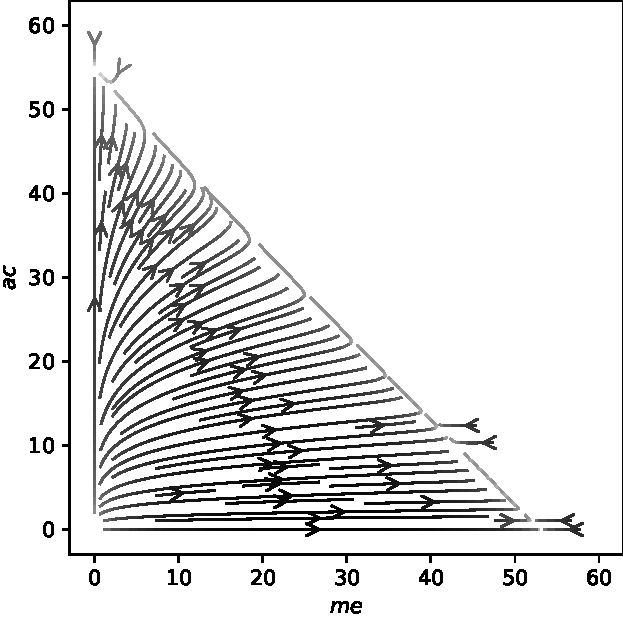
\includegraphics[width=\textwidth]{vectorfield_noncooperative_assymetric_monostable_ac.pdf}
                    \caption*{\small \textbf{(a)}}
                \end{minipage}
                \begin{minipage}{0.3\textwidth}
                    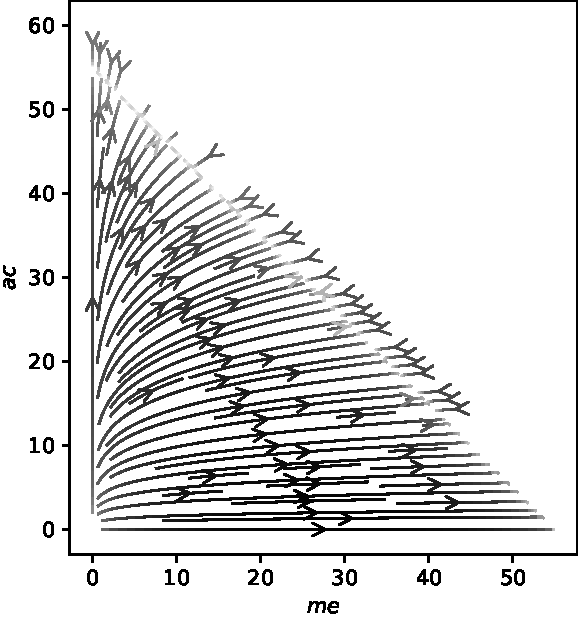
\includegraphics[width=\textwidth]{vectorfield_noncooperative_asymmetric_multistable.pdf}
                    \caption*{\small \textbf{(b)}}
                \end{minipage}
                \begin{minipage}{0.3\textwidth}
                    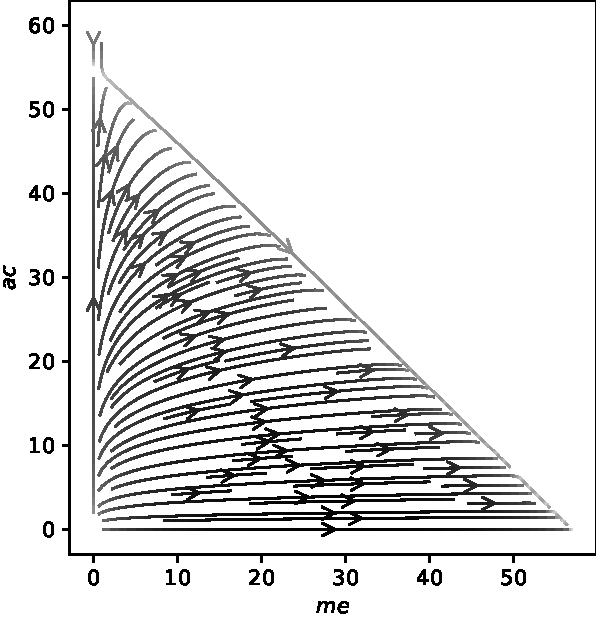
\includegraphics[width=\textwidth]{vectorfield_noncooperative_assymetric_monostable_me.pdf}
                    \caption*{\small \textbf{(c)}}
                \end{minipage}
               \caption{Vector fields describing the non-cooperative 60 nucleosome system with varying enzyme rates. These mainly define the parameters $\alpha_n$ and $\beta_n$ if the enzyme types are constant. The axes describe in absolute numbers the occurrence of methylation (x-axis) and acetylation (y-axis). \textbf{(a)} describes the case for $\nicefrac{\alpha_1}{\alpha_2} > \nicefrac{\beta_1}{\beta_2}$ resulting in a separatrix with gradient towards $(0,N(1-\nicefrac{\beta_1}{\beta_2}))$. In \textbf{(b)}, the equality $\nicefrac{\alpha_1}{\alpha_2} = \nicefrac{\beta_1}{\beta_2}$ results in a zero-gradient separatrix. In \textbf{(c)}, $\nicefrac{\alpha_1}{\alpha_2} < \nicefrac{\beta_1}{\beta_2}$ results in a separatrix with gradient towards $(N(1-\nicefrac{\alpha_1}{\alpha_2}),0)$. From Mayer in \cite{mayer2020langevin}.}
               \label{img:nonCooperativeVectorFields}
            \end{figure}
            %

            %
            One could argue, that for the case of $\nicefrac{\alpha_1}{\alpha_2} = \nicefrac{\beta_1}{\beta_2}$, the zero-gradient separatrix interpreted as a set of points fulfilling a linear equation presents an infinite amount of stable points, thus rendering this specific system multistable. However, one point on the separatrix can hardly be described stable, because it is not resistant to small perturbations. In fact, even the most atomic displacement, namely the state change of one nucleosome, most likely leads to another point on the separatrix and not forcibly to the previous one. Thus, the separatrix as a whole, containing both non-trivial fix points can be described as stable and disqualifies every other point on the separatrix from individual stability in the case of $\nicefrac{\alpha_1}{\alpha_2} = \nicefrac{\beta_1}{\beta_2}$, hence the monostable nature of all the systems in fig. \ref{img:nonCooperativeVectorFields}.
            %


        \subsection{Bi- and multistable states}
            \label{subsec:multistable}
            %
            In order for a dynamic histone PTM system to be bistable, the enzymes have to show cooperativity \cite{dodd2011barriers,sneppen2019theoretical,mayer2020langevin}. According to Sneppen \cite[][p.48]{sneppen2014models}, \enquote{cooperative binding means that the probability of occupying a state increases more than linearly with the concentrations of the binding molecules}.
            %

            %
            In \cite{dodd2011barriers}, Dodd et al. specify the nature of cooperativity in order to reach ultrasensitivity\footnote{From Dodd et al. \cite{dodd2011barriers}: \enquote{Ultrasensitivity is a nonlinearity that magnifies any numerical advantage of one nucleosome type over another, allowing positive feedback to strongly push the system away from intermediate states and towards a large majority of one or other type.}} and thus a robustly bistable system as follows\footnote{citations inside the quote changed their appearance in order to remain functional and to stylistically fit this work}:
            %

            %
            \begin{quote}
                “Cooperativity can be direct, where two modified nucleosomes act together to recruit an enzyme to modify a third nucleosome \cite{3dodd2007theoretical,11sedighi2007epigenetic,15micheelsen2010theory}, or indirect, where each modified nucleosome catalyzes one of two separate modification reactions to fully convert a third nucleosome \cite{3dodd2007theoretical,13david2009inheritance}. A critical requirement for ultrasensitivity is that modified nucleosomes must act nonlocally, stimulating modification of nucleosomes located some distance away on the DNA. This long-range interaction is necessary for any nucleosome to be able to ‘sense’ the majority nucleosome type within the patch and cannot be provided by simple neighbor-to-neighbor contact \cite{3dodd2007theoretical,15micheelsen2010theory}.”
            \end{quote}
            %

            %
            Thus, for single enzymes, direct cooperativity can only be a property of those enzymes which read at least three nucleosomes. Indirect cooperativity can be achieved in a two-step process which involves two enzymes that each read at least two nucleosomes.
            %

            %
            In order to reach robust bistability, the “read-only” nucleosomes should not be direct neighbours of the nucleosome to be (un)modified, as is the case in Dodd et al.'s model where every nucleosome is able to "see" each other one, which they justify by biological phenomena such as higher order chromatin structure or DNA looping \cite{dodd2007theoretical}. This non-local interaction allows the modification that is superiorly prevalent over the whole string at that moment to be accounted for and recognized by the enzymes.
            %

            %
            It is important to stress that cooperativity is not imperatively necessary in order for a system to be bistable \cite{dodd2007theoretical}. However, according to Dodd et al., the absence of cooperativity makes bistability hard to achieve, hardly robust and only possible under conditions, where there are very low noise levels within the system.
            %

            %
            On a sidenote, the definition of cooperativity given by Dodd et al. might seem slightly counterintuitive from a biochemical point of view, where the notion of cooperativity is strongly associated to be an asset of the enzyme \cite{cooperativityDefBritannica}. In contrast, according to Dodd et al., cooperativity is described as a property of a set of nucleosomes being able to “cooperate” in order to recruit an enzyme and catalyse a reaction. A biochemist might be more comfortable with the enzymes being the active part in the system and most notably the catalyst of the occurring reactions instead of the nucleosomes, which most definitely do not catalyse any chemical reaction. As a consequence, in this work, direct cooperativity will be defined as a property of cooperative enzymes whereas indirect cooperativity involves a set of two non-cooperative enzymes.
            %

            %
            Even though the biochemical implications were not ideally put, the mathematical implications explained by Dodd et al. are untouched from these imprecisions.\\
            %

            %
            Mayer in \cite{mayer2020langevin} expressed the time dependent concentration of the modifications on the nucleosome string with cooperative modification adders and non-cooperative modification removers in the CME system depicted in eqns. \ref{eqn:cooperative}.
            %

            %
            \begin{subequations}
                \begin{align}
                    &\frac{\partial a}{\partial t} = \underbrace{- \alpha_1 a }_{\textrm{ac removal}} + \underbrace{ \alpha_2 N^2 a^2 (1-a-m) }_{\textrm{ac addition (cooperative)}}\\
                    &\frac{\partial m}{\partial t} = \underbrace{- \beta_1 m }_{\textrm{me removal}} + \underbrace{ \beta_2 N^2 m^2 (1-a-m) }_{\textrm{me addition (cooperative)}}
                \end{align}
                \label{eqn:cooperative}
            \end{subequations}
            %

            %
            This cooperative system is now cubic in both dimensions and exhibits thus up to 9 critical points. Some of these can quite easily be identified graphically.
            %

            %
            Fig. \ref{img:cooperativeVectorField} depicts the vector field of a system with random and cooperative enzymes at symmetrical rates for methylation and acetylation. Some critical values can clearly be identified. They are summarized in tab. \ref{tab:cooperativeCriticalValues}.
            %

            %
            \begin{figure}[htbp!]
                \centering
                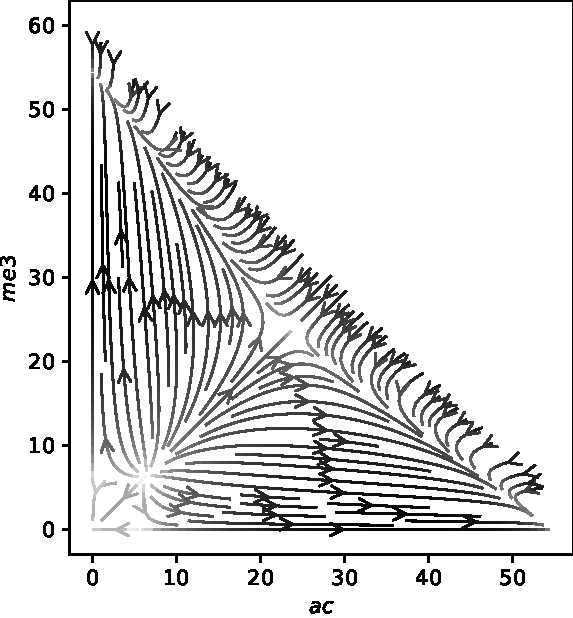
\includegraphics[width=.5\textwidth]{vectorfield_cooperative.pdf}
                \caption{Vector fields describing the cooperative 60 nucleosome system with varying enzyme rates. These mainly define the parameters $\alpha_n$ and $\beta_n$ if the enzyme types are constant. The axes describe in absolute numbers the occurrence of acetylation (x-axis) and methylation (y-axis). From \cite{mayer2020langevin}.}
                \label{img:cooperativeVectorField}
            \end{figure}
            %

            %
            \begin{table}[htbp!]
                \caption{Critical values in $(a,m)$ notation as identified graphically in fig. \ref{img:cooperativeVectorField}.}
                \begin{center}
                    \begin{tabular}{l r}
                        \hline
                        \textbf{critical point} & \textbf{stability} \\
                        \hline
                        $(0,0)$     & stable \\
                        $(8,8)$     & unstable \\
                        $(0,5)$     & unstable \\
                        $(5,0)$     & unstable \\
                        $(0,55)$    & stable \\
                        $(55,0)$    & stable \\
                        $(25,25)$   & saddle point \\
                        \hline
                    \end{tabular}
                \end{center}
                \label{tab:cooperativeCriticalValues}
            \end{table}
            %
        %
        %
        \subsection{Bistable switching}
        \label{sec:TheoBistableSwitching}
        %

        %
        In the context of multistable histone PTM systems, the term of epigenetic switches (explained in \ref{sec:TheoryBivalency}) might become ambiguous.
        %

        %
        On the one hand, as explained before, an epigenetic switch linked to bivalency might describe a three state mechanism: the aforementioned irreversible “ON” and “OFF” states, but also the poised “STANDBY” state \cite{Hoffmann2015BivalencyReview}.
        %

        %
        On the other hand, epigenetic switches might be understood following the analogy of a light switch with the “ON” and “OFF” states being the only possible stable states without any relation to bivalent chromatin at all. A possible application of such a system in the context of evolution has been theoretically discussed in \cite{gomez2019epigenetic}. Given that epimutations (i.e. switching from one stable state to the other) is usually much faster than genetic mutation, the phenotypic diversity and quick adaptation might be an evolutionary advantage in fast fluctuating environments.\\
        %

        %
        Both concepts are relevant to this work. Accordingly, \textit{bistable switching} is hereby explicitly defined as the possibly reversible change from one stable activating or silencing macrostate to the respective other one in absence of an intermediate identifiable “STANDBY” state.
        %

        %
        In contrast, \textit{bivalent switching} is hereby defined as the transition from a pseudostable intermediate (“STANDBY”) state to a stable activating or silencing macrostate within a histone PTM system. Contrarily to the corresponding concept in \cite{Hoffmann2015BivalencyReview}, bivalent switching as defined in the scope of this work is not forcibly irreversible, making bivalent switching more relatable to the given definition of bistable switching.
        %
        %
    %
    %
    %
    %
    \section{Impact of this work}
        %
        Although the mathematical foundation on whether a system can and cannot show bistability was already established, the execution in terms of building a model and rigorously identifying the influence of different factors within the model on the dynamics of a bistable system have, to the knowledge of the author, not been explored yet.
        %

        %
        Also, to date, bistable systems have not yet been modelled by means of a software that takes limited enzyme reach into account, while still allowing non-local interactions, like \ed/ does. This is an important distinction from other models, because neighbour-to-neighbour relations are not neglected, which marks an important step towards real-life chromatin systems.\\
        %

        %
        This thesis will show the potential and limitations of a model with fixed neighbour relations concerning bistability and the switching between stable states throughout the simulation. Furthermore, this work will take a deep look at the working mechanisms of bistability occurring on non-cyclic, as well as cyclic nucleosome strings.
        %
    %
    %
%
%
